\documentclass[12pt,a4paper,titlepage]{article}
\usepackage[utf8]{inputenc}

\usepackage[left=2cm,right=2cm,top=2cm,bottom=2cm]{geometry}
\usepackage{amsmath}
\usepackage{amssymb}
\usepackage{amsthm}
\usepackage{hyperref}
\usepackage{graphicx}
\usepackage[space]{grffile}

\usepackage{listings}
\lstset{language=Java}


\newcommand{\class}[1]{$\mathtt{#1}$}

\author{Jonathan Visbecq, Gaspard Férey}
\title{Projet d'INF 431 \\ - \\ Rapport}


\begin{document}
\maketitle

\section{Hachage}

\begin{figure}
	\centering
	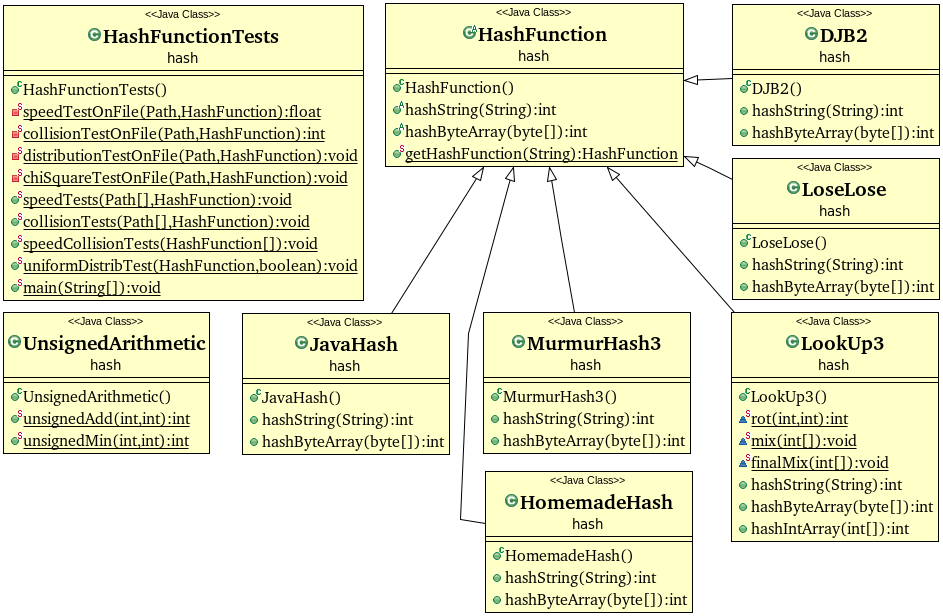
\includegraphics[scale=0.75, angle=90]{../Java Workspace/Test Hash/hashPackage.png}
\end{figure}

Nous avons choisit de définir chacune des fonctions de hachage comme des sous-classes de la classe abstraite \class{HashFunction}.
Ainsi cette classe impose la définition des méthodes suivantes :
\begin{lstlisting}
	public int hashByteArray(byte[] array);
	public int hashString(String s);
\end{lstlisting}
dont l'implémentation dépends, bien sur, de la fonction de hachage et qui implémentent le hachage des types de données qui nous intéressent.

\subsection{Le hachage \class{LookUp3}}
Cette classe implante un hachage tel qu'il est décrit à adresse \href{http://www.burtleburtle.net/bob/c/lookup3.c}{cette adresse}.

\subsection{Le hachage \class{MurmurHash3}}
Cette classe implante un hachage tel qu'il est décrit à adresse \href{http://en.wikipedia.org/wiki/MurmurHash}{cette adresse}.

\subsection{Autres hachages}
Principalement pour les comparer aux deux précédents, nous avons définit d'autres fonctions de hachage moins efficaces :
\begin{itemize}
\item \class{DJB2} dont la description peut être trouvée à \href{http://www.cse.yorku.ca/~oz/hash.html}{cette adresse}.
\item \class{JavaHash}, la fonction de hachage par défaut de Java.
\item \class{LoseLose}, dont la description peut être trouvée à \href{http://www.cse.yorku.ca/~oz/hash.html}{cette adresse}.
\item \class{HomemadeHash} 
\end{itemize}

\subsection{La classe \class{HashFunctionTests}}
Cette classe regroupe les méthodes permettant de comparer et tester les différentes fonctions de hachages.
On y trouve en particulier les méthodes suivantes :
\begin{itemize}

\item \begin{lstlisting}
private static float speedTestOnFile(Path path, HashFunction func)
\end{lstlisting}
Cette fonction parcours le fichier désigné par \class{path} et applique la fonction de hachage \class{func} sur chacun de ses mots. Elle retourne le temps que ce parcours a nécessité (en secondes).

\item \begin{lstlisting}
public static void speedTests(Path[] paths, HashFunction func)
\end{lstlisting}
Cette fonction effectue le même test sur tout les fichiers de \class{paths} et affiche les résultats dans la sortie standard.

\item \begin{lstlisting}
private static int collisionTestOnFile(Path path, HashFunction func)
\end{lstlisting}

\item \begin{lstlisting}
public static void collisionTests(Path[] paths, HashFunction func)
\end{lstlisting}
Cette fonction effectue le même test sur tout les fichiers de \class{paths} et affiche les résultats dans la sortie standard.

\item \begin{lstlisting}
private static void distributionTestOnFile(Path path, HashFunction func)
\end{lstlisting}

\item \begin{lstlisting}
private static void chiSquareTestOnFile(Path path, HashFunction func)
\end{lstlisting}







\end{itemize}









\end{document}